\documentclass[12pt]{article}

\usepackage{graphicx}
\usepackage{paralist}
\usepackage{amsfonts}
\usepackage{hyperref}
\usepackage{upquote}
\usepackage[english]{babel}
\usepackage[autostyle, english = american]{csquotes}

\MakeOuterQuote{"}
\MakeInnerQuote{´}
\oddsidemargin 0mm
\evensidemargin 0mm
\textwidth 150mm
\textheight 200mm
\renewcommand\baselinestretch{1.0}

\pagestyle {plain}
\pagenumbering{arabic}

\newcounter{stepnum}

\title{Environment Set Up Instruction}
\author{Dong Chen}

\begin {document}

\maketitle

This is an instruction to set up the environment in each language to run benchmark tests. The instruction includes set up for 
assembly script, go, rust, and p0. This is a supplement document for the project of class 4tb3/6tb3.

\section{AssemblyScript}
This is the instruction to set up AssemblyScript in your local machines.
\subsection{Step 1: Install AssemblyScript}
In order to run AssemblyScript, you have to set up the environment. The following command will install the Assembly Script 
which is a subset of TypeScript.
~\newline
\begin{verbatim}
npm install -g assemblyscript
\end{verbatim}

\subsection{Step 2: Create a TypeScript file}
Then, create a file with .ts suffix. This a ts file is a TypeScript file. In short, it is a language like Javascript but 
it has data types. The following is the file calculate Fibonacci sequence in TypeScript.
~\newline

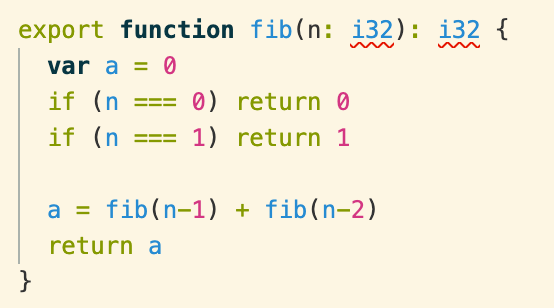
\includegraphics[scale = 0.6]{img/ts-fib}

\subsection{Step 3: Transform TypeScript to WebAssembly}
After creating the TypeScript file, use the following command to transform TypeScript to WebAssembly. asc is the command for 
AssemblyScript.
~\newline
\begin{verbatim}
asc fib.ts -o fib.wasm
\end{verbatim}
~\newline
A wasm file will be created, and it has equivalent methods to its source file.

\subsection{Step 4: Create a html file}
In order to run a wasm file, we can use Javascript via local browsers. The following html file needs to be created, it can 
load the wasm file. Therefore we can use the browser console to test the wasm file.
~\newline

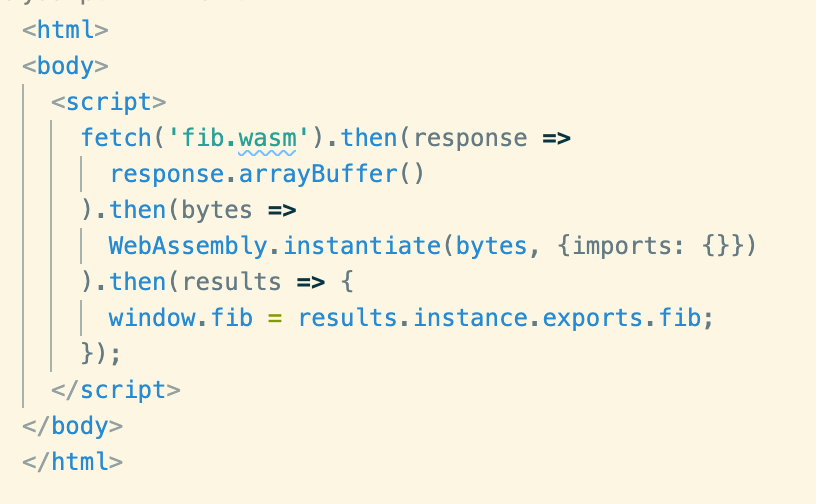
\includegraphics[scale = 0.6]{img/as-html}

\subsection{Step 5: Install http-server}
In order to mimics the host server environment, we have to install http-server package. The following command will install http-server
~\newline
\begin{verbatim}
npm install -g http-server
\end{verbatim}
~\newline
After installation, run http-server by typing http-server in the command line and load the html file.

\subsection{Step 6: Run Webassembly in Browsers}
In the browser console, type fib() to test the outcome. The example shows in the following.
~\newline

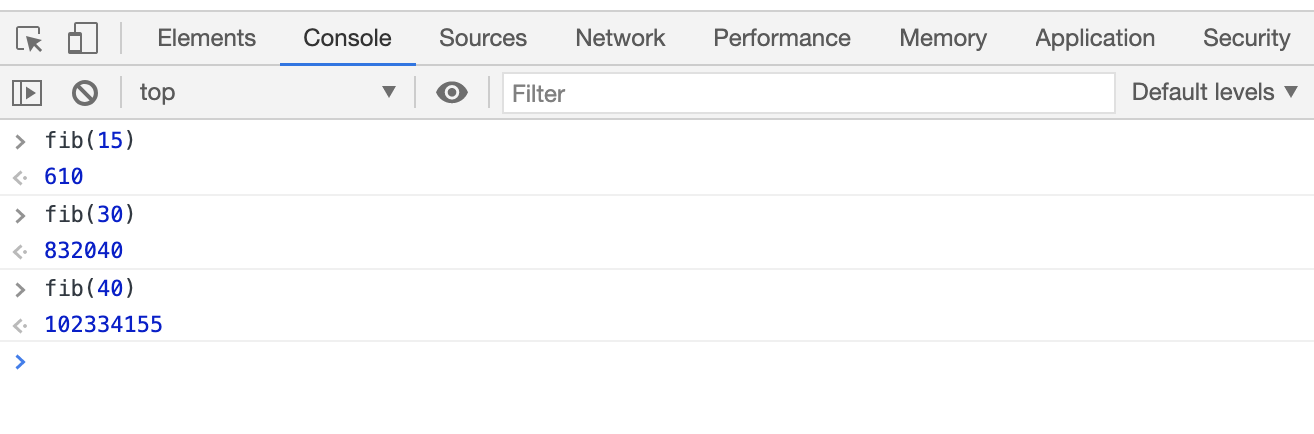
\includegraphics[scale = 0.6]{img/as-browser}

\pagebreak
\section{Go Language}
This is the instruction to set up the Go language in your local machines.

\subsection{Step 1: Install Go language}
There are various ways to install Go. You can reference to \href{https://golang.org/doc/install}{Golang Download and install}
~\newline
The author use brew to install go by using the following command in the command terminal.
~\newline
\begin{verbatim}
brew install go
\end{verbatim}

\subsection{Step 2: Create a Go file}
Then, create a go file. The following is a go file with the Fibonacci sequence. In the following go file, the author exposed the 
fib file, so users can access the fib method in the browser console. Additionally, the go file will read the input which come 
from users and calculate the Fibonacci sequence.
~\newline

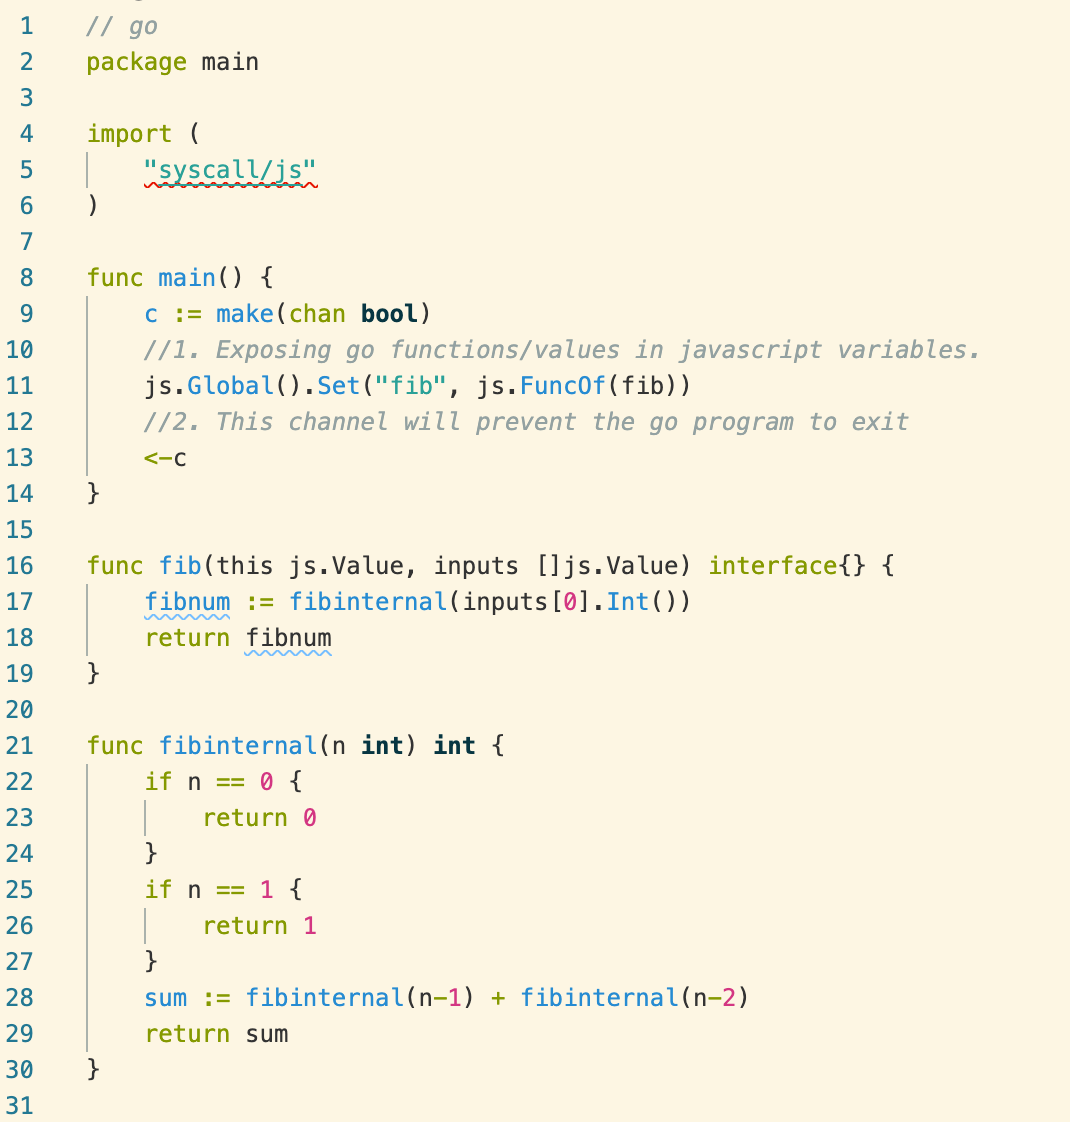
\includegraphics[scale = 0.6]{img/go-fib}

\subsection{Step 3: Compile Go to WebAssembly}
To compile a go file, first, initialize the go mod in the current folder. It will create a .mod file. Then, run the following 
command to start the transformation.
~\newline
\begin{verbatim}
GOOS=js GOARCH=wasm go build -o fib.wasm fib.go
\end{verbatim}
~\newline
A wasm file will be created, and it has equivalent methods to its source file.

\subsection{Step 4: Copy wasm\_exec.js and wasm\_exec.html}
These are two files already provide by Go language, we can reuse them to run webassembly in the local browser. These two files 
locates at (go env GOROOT)/misc/wasm/. Use the command "go env GOROOT" to get the exact root path, and concatenate it with the 
rest of path.
~\newline
Edit the file name in html file to match the wasm name. The following is the html file for this project.
~\newline

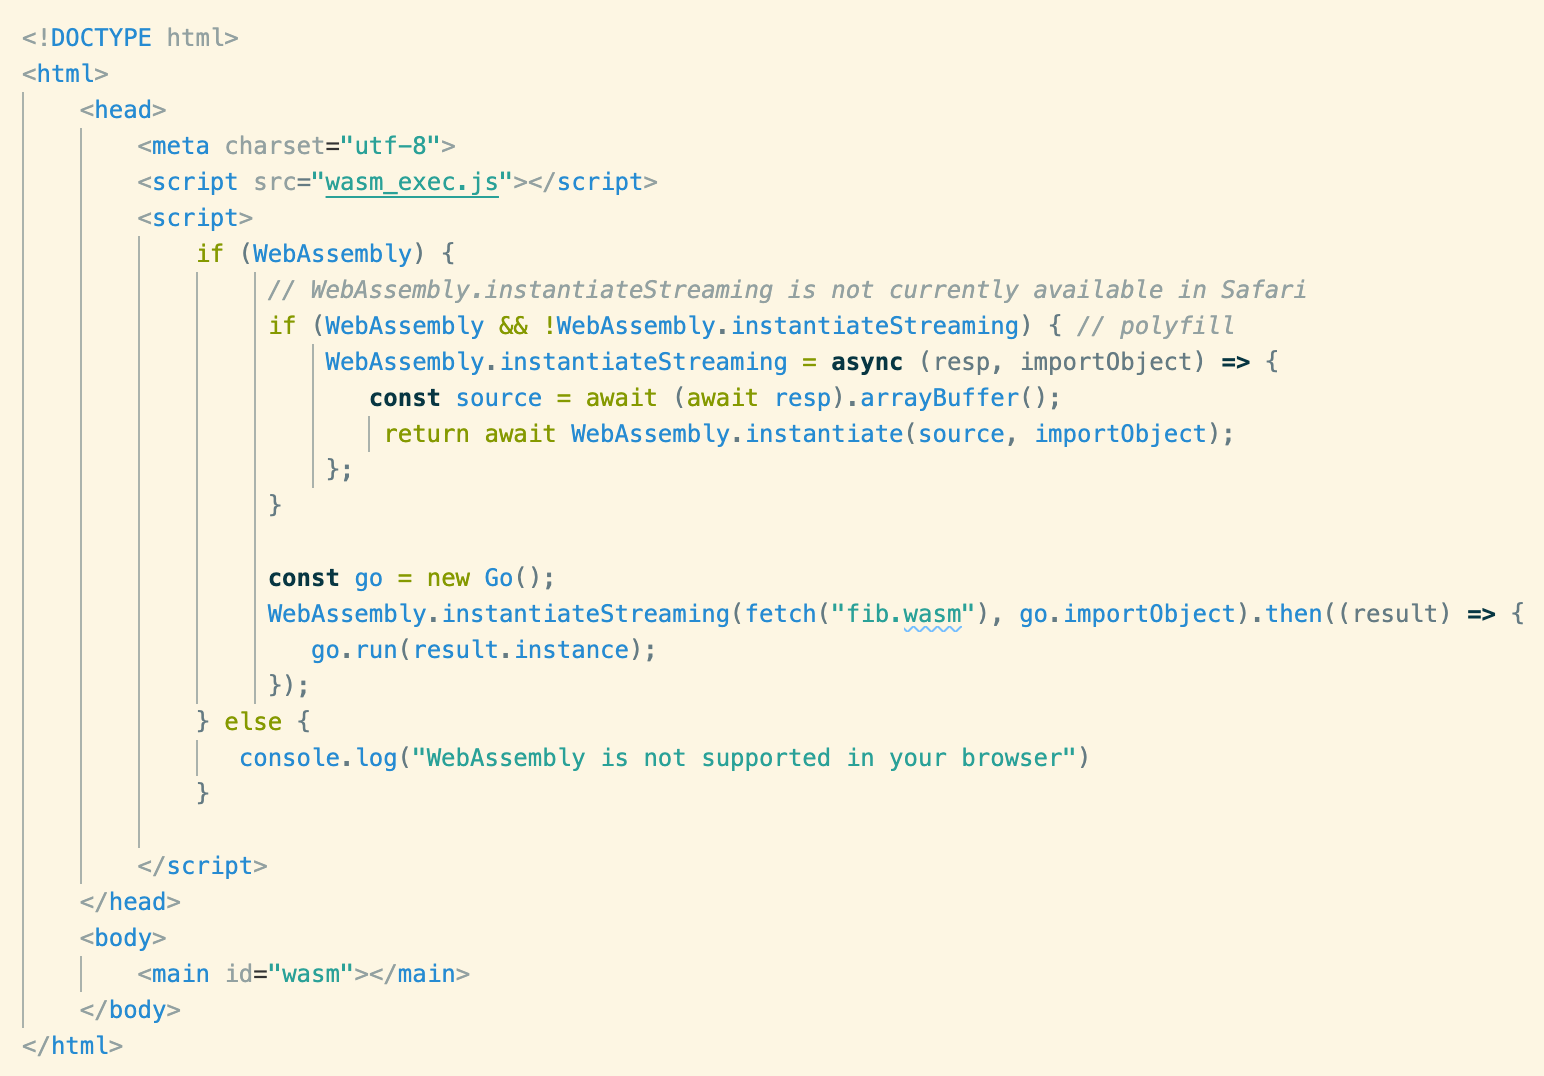
\includegraphics[scale = 0.6]{img/go-html}

\subsection{Step 5: Run Webassembly in Browsers}
In this step, we use the same method in AssemblyScript, using http-server. In the browser console, type fib() to test 
the outcome. The example shows in the following.
~\newline

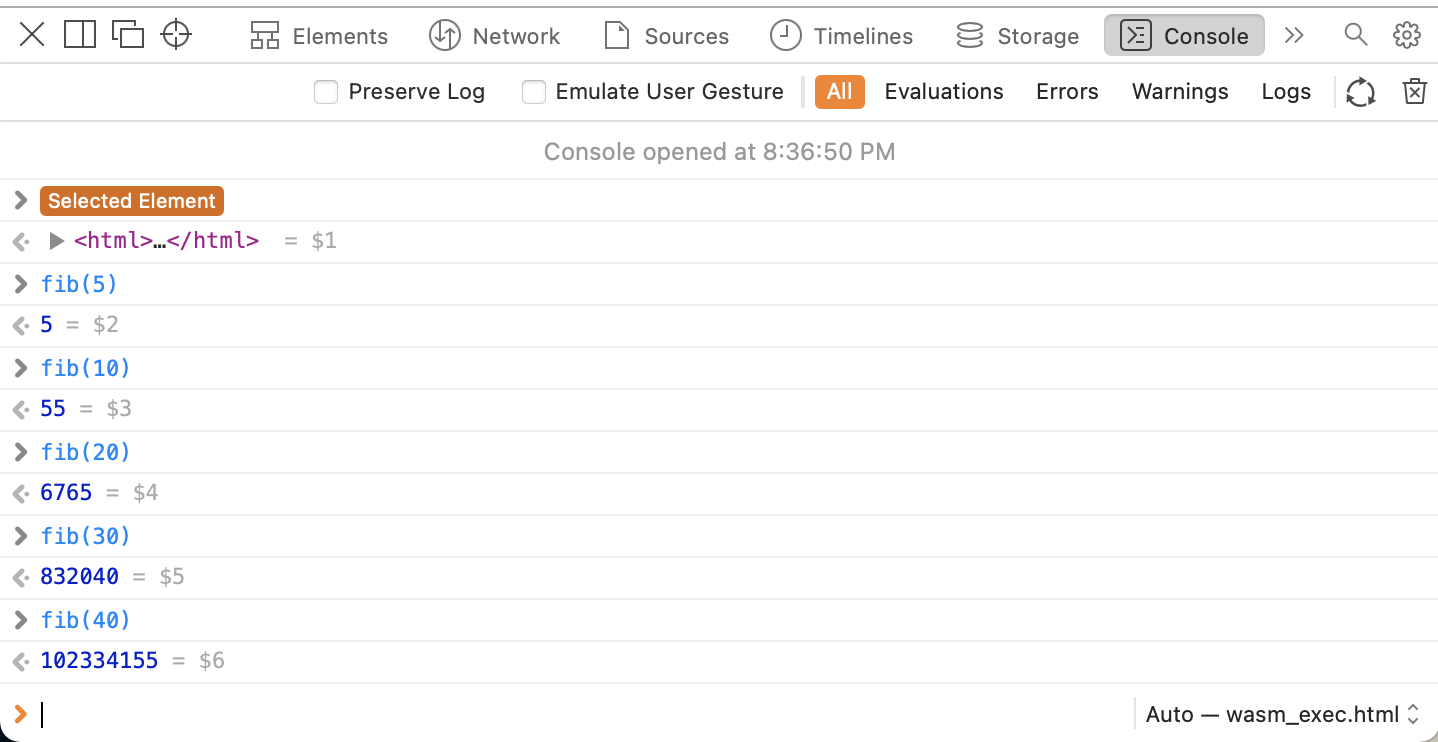
\includegraphics[scale = 0.6]{img/go-browser}

\pagebreak
\section{Rust Language}
This is the instruction to set up the Rust language in your local machines.

\subsection{Step 1: Install Rust Language}
There are various ways to install Go. You can reference to \href{https://doc.rust-lang.org/book/ch01-01-installation.html}{Rust Installation}
~\newline
The author uses the following installed Rust in the command terminal.
~\newline
\begin{verbatim}
curl --proto '=https' --tlsv1.2 https://sh.rustup.rs -sSf | sh
\end{verbatim}

\subsection{Step 2: Create a Rust file}
Then, create a rust file. The following is a rust file with the Fibonacci sequence.
~\newline

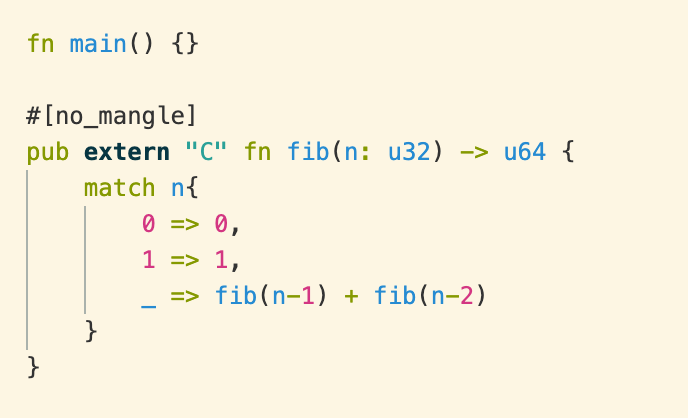
\includegraphics[scale = 0.6]{img/rust-fib}

\subsection{Step 3: More Packages}
There is one more package that need to be installed. Run the following to install the required target.
~\newline
\begin{verbatim}
rustup target add wasm32-unknown-unknown --toolchain nightly
\end{verbatim}

\subsection{Step 4: Compile Go to WebAssembly}
To compile a go file, run the following command to start the transformation.
~\newline
\begin{verbatim}
rustc +nightly --target wasm32-unknown-unknown -O fib.rs
\end{verbatim}
~\newline
A wasm file will be created, and it has equivalent methods to its source file.

\subsection{Step 5: Create a html file}
A html needs to be created to load wasm locally. This is a similar implementation in AssemblyScript step 4.

\subsection{Step 6: Run Webassembly in Browsers}
In this step, we use the same method in AssemblyScript, using http-server. In the browser console, type fib() to test 
the outcome. The example shows in the following.
~\newline

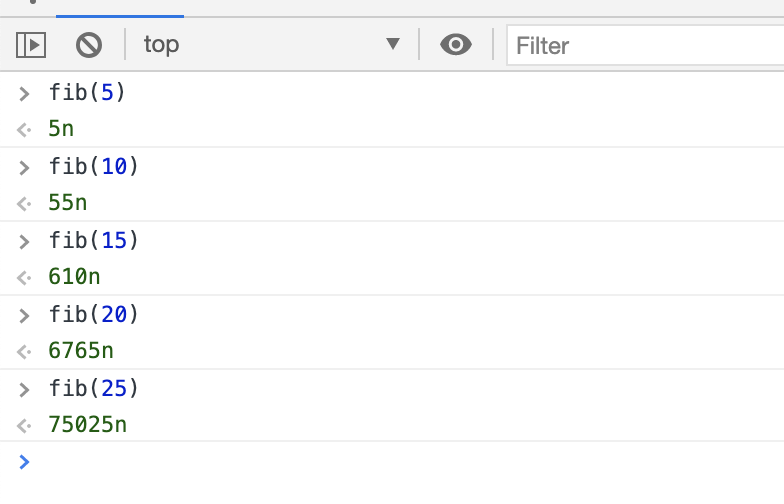
\includegraphics[scale = 0.6]{img/rust-browser}

\pagebreak
\section{P0 Language}
P0 language has been taught in the class. Please refer to chapter 5 on how to set up the P0 
language.

\pagebreak
\section{Reference}
\begin{itemize}
    \item \href{https://medium.com/@BenedekGagyi/the-simplest-way-to-get-started-with-webassembly-1f92f6f90d24}{The simplest way to get started with WebAssembly}
    \item \href{https://medium.com/swlh/getting-started-with-webassembly-and-go-by-building-an-image-to-ascii-converter-dea10bdf71f6}{Getting Started With WebAssembly and Go By Building an Image to ASCII Converter}
    \item \href{https://www.hellorust.com/setup/wasm-target/}{Rust for the Web}
\end{itemize}

\end {document}
